% Editable vector illustration. Observations and decisions are conceptual.
\documentclass[tikz,border=3pt]{standalone}
\usepackage[T1]{fontenc}
\usepackage{times}
\usepackage{amsmath}
\usetikzlibrary{arrows.meta,calc}
\definecolor{ink}{HTML}{22364A}
\definecolor{muted}{HTML}{617182}
\definecolor{edge}{HTML}{D9E3EB}
\definecolor{blue}{HTML}{527696}
\definecolor{bluepale}{HTML}{F3F7FB}
\definecolor{teal}{HTML}{287E75}
\definecolor{tealpale}{HTML}{EEF8F4}
\definecolor{amber}{HTML}{BC803B}
\definecolor{amberpale}{HTML}{FFF5E7}
\definecolor{purple}{HTML}{776AA4}
\definecolor{purplepale}{HTML}{F4F1FA}
\definecolor{skin}{HTML}{F1CFB5}
\tikzset{
  txt/.style={text=ink,font=\fontsize{12}{14}\selectfont,inner sep=0pt,align=left},
  secondary/.style={txt,font=\fontsize{11}{13}\selectfont,text=muted},
  heading/.style={txt,font=\bfseries\fontsize{13}{15}\selectfont},
  box/.style={rounded corners=5pt,line width=.7pt,draw=edge,fill=white},
  arrow/.style={-{Stealth[length=2.0mm,width=1.4mm]},draw=muted,line width=1pt},
  flow/.style={line width=1.15pt,rounded corners=3pt}
}
\newcommand{\walker}[2]{%
  \begin{scope}[shift={(#1,#2)},line cap=round,line join=round]
    \fill[skin] (0,-.48) circle (.105);
    \draw[ink,line width=1.2pt] (-.07,-.54) to[bend left=32] (.075,-.54);
    \draw[teal,line width=3.6pt] (-.025,-.32)--(-.09,.04);
    \draw[teal,line width=1.55pt] (-.03,-.28)--(.15,-.08)--(.32,-.10);
    \draw[teal,line width=1.55pt] (-.055,-.24)--(-.23,-.07)--(-.31,.06);
    \draw[ink,line width=1.9pt] (-.09,.04)--(.07,.25)--(.25,.39);
    \draw[ink,line width=1.9pt] (-.09,.04)--(-.23,.27)--(-.32,.41);
    \draw[ink,line width=1.5pt] (.23,.4)--(.34,.4);
    \draw[ink,line width=1.5pt] (-.32,.42)--(-.22,.42);
  \end{scope}}
\newcommand{\calendarwalk}[4]{%
  \path[box] (#1,.97) rectangle ++(2.72,1.53);
  \path[fill=tealpale,rounded corners=5pt] (#1,.97) rectangle ++(2.72,.40);
  \fill[tealpale] (#1,1.20) rectangle ++(2.72,.17);
  \node[txt,text=teal,font=\bfseries\fontsize{11}{13}\selectfont,anchor=west]
    at (#1+.18,1.16) {#2};
  \draw[teal,line width=1.5pt,line cap=round] (#1+.37,.90)--(#1+.37,1.07);
  \draw[teal,line width=1.5pt,line cap=round] (#1+2.34,.90)--(#1+2.34,1.07);
  \walker{#1+.52}{1.99}
  \ifnum#4=1
    \node[txt,anchor=west] at (#1+1.02,1.68) {Walking};
    \node[secondary,anchor=west] at (#1+1.02,2.16) {#3};
  \else
    \node[txt,anchor=west] at (#1+1.02,1.93) {#3};
  \fi
}
% Both agents use the exact same bounded event strip.
\newcommand{\recentstrip}[1]{%
  \path[box] (#1,4.32) rectangle ++(8.05,1.21);
  \node[txt,font=\bfseries\fontsize{11.5}{13}\selectfont,anchor=west]
    at (#1+.25,4.65) {Recent events};
  \draw[edge,line width=1pt] (#1+.25,5.13)--(#1+7.65,5.13);
  \path[fill=blue!9,rounded corners=1.1pt] (#1+.26,4.99) rectangle ++(.27,.28);
  \path[fill=blue!15,rounded corners=1.1pt] (#1+.67,4.99) rectangle ++(.27,.28);
  \fill[white] (#1+1.09,4.93) rectangle ++(.29,.40);
  \draw[muted!65,line width=.85pt] (#1+1.10,5.32)--(#1+1.24,4.94);
  \draw[muted!65,line width=.85pt] (#1+1.25,5.32)--(#1+1.39,4.94);
  \foreach \step in {0,...,5}{
    \path[fill=blue!35,rounded corners=1.2pt]
      (#1+1.71+\step*.94,4.94) rectangle ++(.38,.38);
  }
  \path[fill=amber,rounded corners=1.2pt] (#1+7.23,4.91) rectangle ++(.44,.44);
}
\newcommand{\miniday}[2]{%
  \path[draw=teal!35,fill=tealpale,rounded corners=1.8pt,line width=.6pt]
    (#1,6.62) rectangle ++(.78,.53);
  \node[txt,text=teal,font=\bfseries\fontsize{7}{8}\selectfont,anchor=center]
    at (#1+.39,6.78) {#2};
  \draw[teal!20,line width=1pt] (#1+.12,7.00)--(#1+.67,7.00);
  \draw[teal,line width=2.2pt,line cap=round] (#1+.33,7.00)--(#1+.57,7.00);
}
\begin{document}
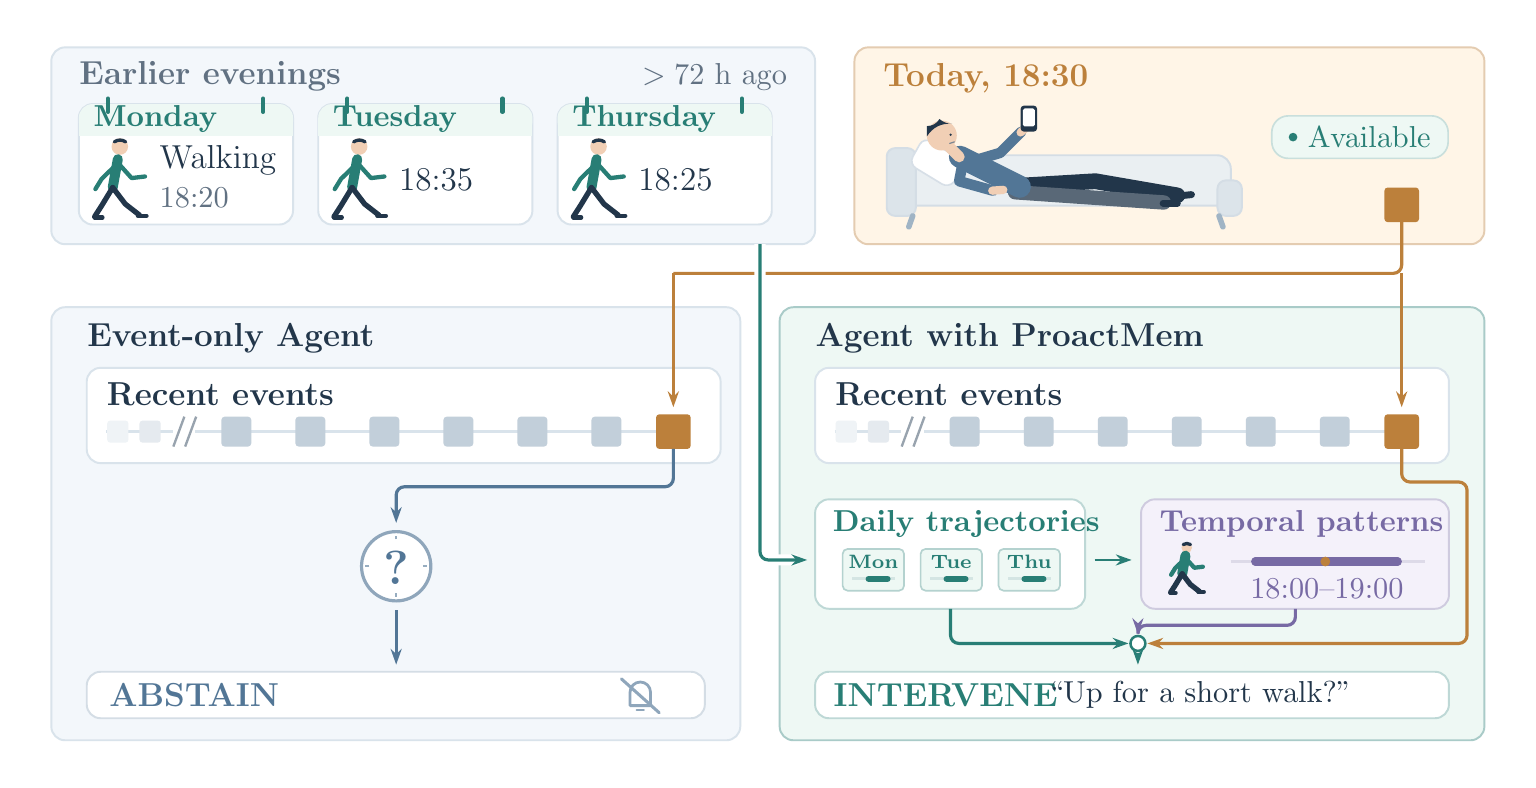
\begin{tikzpicture}[x=1cm,y=-1cm]
  \path[use as bounding box] (0,0) rectangle (18.8,9.3);
  \fill[white] (0,0) rectangle (18.8,9.3);

  % Historical observations are outside the bounded recent-event view.
  \path[box,fill=bluepale] (.30,.25) rectangle (10.0,2.75);
  \node[heading,text=muted,anchor=west] at (.65,.62) {Earlier evenings};
  \node[secondary,anchor=east] at (9.65,.62) {$>72$ h ago};
  \calendarwalk{.65}{Monday}{18:20}{1}
  \calendarwalk{3.69}{Tuesday}{18:35}{0}
  \calendarwalk{6.73}{Thursday}{18:25}{0}

  \path[box,draw=amber!40,fill=amberpale] (10.5,.25) rectangle (18.5,2.75);
  \node[heading,text=amber,anchor=west] at (10.86,.64) {Today, 18:30};

  % Awake reclining user: cushion, extended legs, open eye, and raised phone.
  \begin{scope}[line cap=round,line join=round]
    \path[fill=blue!12,draw=blue!25,rounded corners=5pt,line width=.7pt]
      (11.02,1.62) rectangle (15.28,2.26);
    \path[fill=blue!20,draw=blue!25,rounded corners=3pt,line width=.7pt]
      (10.91,1.53) rectangle (11.28,2.39);
    \path[fill=blue!20,draw=blue!25,rounded corners=3pt,line width=.7pt]
      (15.11,1.94) rectangle (15.42,2.39);
    \draw[blue!55,line width=2pt] (11.24,2.39)--(11.19,2.53);
    \draw[blue!55,line width=2pt] (15.13,2.39)--(15.18,2.53);
    \path[fill=white,draw=blue!23,rounded corners=3pt,line width=.6pt]
      (11.19,1.73)--(11.38,1.39)--(11.94,1.73)--(11.70,2.04)--cycle;
    \draw[ink,line width=5.7pt] (12.55,2.01)--(13.56,1.95)--(14.60,2.13);
    \draw[ink!75,line width=5.2pt] (12.54,2.09)--(13.55,2.16)--(14.43,2.22);
    \draw[ink,line width=2.5pt] (14.59,2.14)--(14.78,2.12);
    \draw[ink,line width=2.5pt] (14.42,2.23)--(14.60,2.23);
    \draw[blue,line width=8pt] (11.84,1.64)--(12.60,2.02);
    \draw[blue,line width=3.8pt] (11.88,1.69)--(11.83,1.95)--(12.26,2.07);
    \draw[skin,line width=3pt] (12.25,2.07)--(12.39,2.06);
    \draw[blue,line width=3.8pt] (11.98,1.70)--(12.35,1.59)--(12.62,1.32);
    \draw[skin,line width=3pt] (12.61,1.33)--(12.68,1.27);
    \draw[skin,line width=4pt] (11.83,1.64)--(11.69,1.50);
    \fill[skin] (11.61,1.37) circle (.19);
    \path[fill=ink] (11.42,1.38) to[bend left=30] (11.74,1.22)
      to[bend left=20] (11.58,1.16) to[bend left=28] (11.42,1.25)--cycle;
    \fill[ink] (11.72,1.36) circle (.016);
    \draw[ink!60,line width=.45pt] (11.71,1.47) to[bend right=20] (11.77,1.45);
    \path[fill=ink,rounded corners=1.2pt] (12.61,.99) rectangle (12.82,1.32);
    \path[fill=white,rounded corners=.6pt] (12.64,1.025) rectangle (12.79,1.255);
  \end{scope}
  \path[fill=tealpale,draw=teal!25,rounded corners=6pt,line width=.6pt]
    (15.80,1.12) rectangle (18.04,1.66);
  \fill[teal] (16.07,1.39) circle (.055);
  \node[txt,text=teal,font=\fontsize{11}{13}\selectfont,anchor=west]
    at (16.25,1.39) {Available};
  \path[fill=amber,rounded corners=1.2pt] (17.23,2.03) rectangle ++(.44,.44);

  % Equal input representations isolate the visible memory contrast.
  \path[box,fill=bluepale] (.30,3.55) rectangle (9.05,9.05);
  \path[box,draw=teal!40,fill=tealpale] (9.55,3.55) rectangle (18.5,9.05);
  \node[heading,anchor=west] at (.75,3.94) {Event-only Agent};
  \node[heading,anchor=west] at (10.0,3.94) {Agent with ProactMem};
  \recentstrip{.75}
  \recentstrip{10.0}

  % The orange current event branches into both recent-event strips.
  \draw[flow,draw=amber] (17.45,2.47)--(17.45,3.12)--(8.20,3.12);
  \draw[arrow,draw=amber] (8.20,3.12)--(8.20,4.82);
  \draw[arrow,draw=amber] (17.45,3.12)--(17.45,4.82);

  % White bridge: history and current-event paths cross without joining.
  \draw[arrow,flow,draw=teal,preaction={draw=white,line width=4pt}]
    (9.30,2.75)--(9.30,6.76)--(9.90,6.76);

  % Event-only: timing uncertainty and a silent output.
  \draw[arrow,flow,draw=blue] (8.20,5.35)--(8.20,5.83)--(4.68,5.83)--(4.68,6.29);
  \draw[draw=blue!65,line width=1.15pt,fill=white] (4.68,6.84) circle (.44);
  \foreach \a in {0,90,180,270}{
    \draw[blue!60,line width=.65pt]
      ($(4.68,6.84)+(\a:.34)$)--($(4.68,6.84)+(\a:.39)$);
  }
  \node[txt,text=blue,font=\bfseries\fontsize{19}{20}\selectfont,anchor=center]
    at (4.68,6.86) {?};
  \draw[arrow,draw=blue] (4.68,7.40)--(4.68,8.09);
  \path[box,draw=blue!25] (.75,8.18) rectangle (8.60,8.77);
  \node[txt,text=blue,font=\bfseries\fontsize{12}{14}\selectfont,anchor=west]
    at (1.03,8.48) {ABSTAIN};
  \begin{scope}[shift={(7.78,8.48)},line cap=round,line join=round]
    \draw[blue!65,line width=1pt] (-.13,.13)--(-.13,-.04)
      arc[start angle=180,end angle=360,radius=.13]--(.13,.13)--cycle;
    \draw[blue!65,line width=.8pt] (-.045,.19)--(.045,.19);
    \draw[blue!65,line width=1.1pt] (-.24,-.21)--(.24,.22);
  \end{scope}

  % Daily records become an applicable recurring interval.
  \path[box,draw=teal!30] (10.0,5.99) rectangle (13.43,7.38);
  \node[txt,text=teal,font=\bfseries\fontsize{11}{13}\selectfont,anchor=west]
    at (10.22,6.30) {Daily trajectories};
  \miniday{10.35}{Mon}
  \miniday{11.34}{Tue}
  \miniday{12.33}{Thu}
  \draw[arrow,draw=teal] (13.55,6.76)--(14.02,6.76);
  \path[box,draw=purple!35,fill=purplepale] (14.14,5.99) rectangle (18.05,7.38);
  \node[txt,text=purple,font=\bfseries\fontsize{11}{13}\selectfont,anchor=west]
    at (14.37,6.30) {Temporal patterns};
  \begin{scope}[shift={(14.72,6.91)},scale=.64]
    \walker{0}{0}
  \end{scope}
  \draw[draw=purple!25,line width=1.2pt] (15.28,6.78)--(17.74,6.78);
  \draw[draw=purple,line width=3pt,line cap=round] (15.59,6.78)--(17.40,6.78);
  \fill[amber] (16.48,6.78) circle (.062);
  \node[txt,text=purple,font=\fontsize{10.5}{12}\selectfont,anchor=center]
    at (16.5,7.12) {18:00--19:00};

  % Recent context, daily records, and the applicable pattern meet at decision time.
  \draw[arrow,flow,draw=amber] (17.45,5.35)--(17.45,5.77)--(18.28,5.77)
    --(18.28,7.82)--(14.22,7.82);
  \draw[arrow,flow,draw=teal] (11.72,7.38)--(11.72,7.82)--(13.98,7.82);
  \draw[arrow,flow,draw=purple] (16.1,7.38)--(16.1,7.59)--(14.1,7.59)--(14.1,7.70);
  \fill[white,draw=teal,line width=.9pt] (14.1,7.82) circle (.095);
  \draw[arrow,draw=teal] (14.1,7.94)--(14.1,8.09);
  \path[box,draw=teal!30] (10.0,8.18) rectangle (18.05,8.77);
  \node[txt,text=teal,font=\bfseries\fontsize{12}{14}\selectfont,anchor=west]
    at (10.23,8.48) {INTERVENE};
  \node[txt,font=\fontsize{11}{13}\selectfont,anchor=west]
    at (12.95,8.48) {\textquotedblleft Up for a short walk?\textquotedblright};
\end{tikzpicture}
\end{document}
